\documentclass[a4paper,12pt]{article}
\usepackage[utf8]{inputenc}
\usepackage[french]{babel}
\usepackage[T1]{fontenc}
\usepackage{verbatim}
\usepackage{graphicx}
\usepackage{amsmath}
\usepackage{amsfonts}
\usepackage{textcomp}
\usepackage{fullpage}
\usepackage{algorithm2e}
\usepackage{caption}
\usepackage{color}
\usepackage{subcaption}
\usepackage{fancyvrb}
\fvset{commandchars=\\\{\}}
\usepackage[usenames,dvipsnames]{xcolor}
\frenchbsetup{ReduceListSpacing=false,CompactItemize=false}

\title{Recherches et réalisations relatives à une plateforme de
       collaboration estudiantine}
\author{Draft}

\begin{document}

\abovedisplayskip=1pt plus 0pt minus 0pt
\abovedisplayshortskip=6pt plus 3pt
\belowdisplayskip=9pt plus 3pt minus 9pt
\belowdisplayshortskip=9pt plus 3pt minus 4pt

\setlength{\voffset}{-20pt}

\begin{titlepage}
\begin{center}

\begin{minipage}{2in}
	\begin{flushleft}
		\textsf{\small{
		Faculté des Sciences\\
		Département d'Informatique}}
	\end{flushleft}
\end{minipage}
\begin{minipage}{4in}
	\begin{flushright}
		
\includegraphics[scale=0.20]{imgs/ulb2.pdf}
	\end{flushright}
\end{minipage}

\vspace{120pt}

{\Large \bfseries Recherches et réalisations relatives à une plateforme de
       collaboration estudiantine}

\vspace{20pt}

\large{X \textsc{X}}

\vspace{90pt}


\includegraphics[scale=0.6]{imgs/ulb1.pdf}
\end{center}
\end{titlepage}

\setlength{\footskip}{40pt}

\abovedisplayskip=9pt plus 3pt minus 9pt
\abovedisplayshortskip=6pt plus 3pt
\belowdisplayskip=9pt plus 3pt minus 9pt
\belowdisplayshortskip=9pt plus 3pt minus 4pt
\setlength{\parskip}{0.5ex plus 0.2ex minus 0.2ex}
\setlength{\parindent}{0pt}

\newpage
\setlength{\voffset}{0pt}
\setcounter{tocdepth}{2}
\addcontentsline{toc}{subsection}{Table des matières}
\tableofcontents

\newpage

\section{Introduction}

% Depuis toujours l'entraide et le partage font partie des valeurs fondamentales à l'ULB. Les conseils, astuces, notes de cours et autres documents
% ont pendant de nombreuses années été échangés sur le forum de discussion nommé CandiULB.
% Parallèlement à une diversification des mediums de communication sur internet, le forum est petit-à-petit tombé en désuétude
% pour en 2009 être définitivement abandonné.

Différents groupes de personnes ont tenté de remettre le partage à l'ordre du jour 
au travers d'une plateforme adaptée aux besoins des étudiants. C'est sur cette base que le projet décrit ci-après a vu
le jour avec pour objectif d'atteindre cet idéal.

% FIN COMMENTAIRE SUPPRIMER LE § ci dessous
Pendant de nombreuses années, les étudiants de l'ULB échangèrent des conseils, trucs et astuces,
documents et informations via le forum de discussion nommé CandiULB. Ce dernier est tombé en désuétude et vers 2009,
fut définitivement abandonné.
Différents groupes de personnes ont tenté de remettre le partage à l'ordre du jour 
au travers d'une plateforme adaptée aux besoins des étudiants. Ce projet vise cet idéal.

Durant le courant de l'année académique 2010-2011, une série de spécifications ont été écrites,
principalement autour du texte fondateur écrit par Laurent Peuch
\footnote{http://worlddomination.be/blog/2012/idee-dun-plateforme-dentre-aide-pour-edutiants.html}.
Durant l'année académique 2011-2012, ce projet fut mis en place, pour culminer en mai 2012
par la mise en production de la première version de la plateforme étudiante hebergée sur le site du Cercle Informatique
\footnote{https://cours.cerkinfo.be}. Ce document traite de cette plateforme, de ces caractéristiques et des différentes
aspects envisagés pour atteindre une ébauche de plateforme idéale.

Le but principal de la plateforme est d'offrir aux étudiants un espace pour uploader
des documents, les télécharger ou les visionner en ligne. Un espace de discussion est aussi proposé
afin d'échanger sur les cours et les documents. En plus de ces fonctionnalités de base,
le site permet aux utilisateurs d'attribuer des points aux ressources et discussions,
permettant de les hiérarchiser. Ceci a pour avantage de limiter le travail de modération (les mauvaises
contributions sont rendues invisibles au lieu d'être censurées).

Ce document cherche à couvrir différents aspects de cette plateforme, tout d'abord en
expliquant les choix réalisés pour cette plateforme (section 2) et en présentant
le fonctionnement du \textit{framework} choisi (section3). Il abordera ensuite
les questions d'interaction avec une base de données (section 4) et la manière
de gérer la synchronisation entre les différentes versions des modèles et de
la base de données (section 5). Par après, il s'intéressera au projet en lui-même,
avec une explication de la méthode de déploiement (section 6), la
description des fonctionnalités (section 7) et l'architecture des différents
composant et la manière de les configurés (section 8 et 9). La suite du
document détaille certains points particuliers de la plateforme, comme la traduction (section 10),
le pré-traitement des documents (section 11), la fonction de recherche (section 12)
et l'authentification (section 13). Ce document abordera des questions d'ordre 
plus général ainsi que leur traitement par la plateforme. On y trouvera notamment une section sur la
sécurité (section 14) et la validation (section 15). Finalement, ce travail propose aussi
une approche de travail en continuous testing (section 16) et conclura
avec le résultat concret de la plateforme (section 17).


\section{Choix technologiques}

Le projet a été réalisé grâce au \textit{framework} Django, écrit en langage Python.
Python est un langage haut niveau, particulièrement expressif et étudié par
les étudiants en informatique de l'ULB. Un \textit{framework} est une abstraction
fournissant au développeur l'ensemble des bibliothèques, outils et paradigmes
dont il a besoin, lui permettant d'économiser du temps de travail. 

Django fut choisi car il est basé sur un langage étudié à l'ULB et est très populaire.
Ce logiciel joui d'une grande communauté de passionnés, d'une base de documentation
correcte et d'un statut "production-ready". De plus, il est utilisé notamment
par la NASA\footnote{http://science.nasa.gov/}, Instagram
\footnote{http://instagram.com/}
\footnote{http://instagram-engineering.tumblr.com/post/13649370142/what-powers-instagram-hundreds-of-instances-dozens-of}
ou encore The Onion\footnote{http://www.theonion.com/} pour certains de leurs besoins web.


\section{Architecture générale de Django}

Django est un \textit{framework} web dont le langage principal est Python et
dont l'architecture applique les principes de séparation des tâches, inspiré du
modèle MVC. Le but de ce logiciel est de permettre la conception rapide de site
en fournissant une série d'outils et de techniques au développeur. Par exemple,
Django rend transparent l'usage d'une base de données, standardise la manière
d'envoyer une page à l'utilisateur, fournit un système de session et d'authentification,
un système de gestion des logs intégrés...

La liste des fonctionnalités offertes par Django est assez longue, il est malheureusement
impossible d'être exhaustif dans le cadre de ce travail. Les plus importantes
ou celles spécifiquement employées par le projet seront détaillées dans les sections suivantes.

Le protocole HTTP est un protocole sans état (\textit{stateless}), c'est-à-dire
que le client ou le serveur ne peuvent déterminer l'état de l'application client uniquement
sur base de la session HTTP. Cela implique qu'il est possible de traiter chaque requête HTTP
de manière individuelle, sans se soucier de celle présente précedemment ou après. Malheureusement,
pour la majorité des applications il faut aussi mettre en place un mécanisme permettant
d'identifier le client, de garder certaines propriétés de ce dernier...

Chaque requête d'une page web que le client envoie au serveur arrive 
à Django au niveau du résolveur d'URL, première étape sur la figure \ref{fig:mvc}.
Cette étape permet d'associer une fonction
à chaque demande du client. Les URLs sont reconnues au moyen d'expressions rationnelles.
Par exemple, si le développeur veut deux pages web différentes, l'une affichant
le résultat de la fonction \textit{page1} à l'adresse \texttt{http://host/path/index/} et
l'autre affichant le résultat de la fonction \textit{page2} à l'adresse
\texttt{http://host/path/page2/123/}, 123 étant un ID unique, il pourrait employer
le résolveur d'URL suivant :

\begin{verbatim}
urlpatterns = patterns("",
    url(r"^path/index/$", page1),
    url(r"^path/page2/(\d)/$", page2),
)
\end{verbatim}

Le résolveur d'URL permet d'extraire certaines parties de l'URL reconnues et de les donner
comme argument à la fonction à appeler. Dans l'exemple précédent, la fonction \textit{page2}
sera appelée avec le nombre en fin d'URL en argument.

Cette fonction est appelée la \textit{view}. Cette dernière prend au minimum un paramètre,
un objet requête. Il contient énormément d'informations sur le client, l'url demandé,
la méthode HTTP employée, des paramètres du serveur... Le rôle de cette fonction
est de fabriquer la page web envoyée au client, c'est sa valeur de retour. Pour ce faire,
la fonction envoie usuellement des requêtes à la base de données en employant des modèles
d'objet et calcule le rendu de la page en employant le moteur de \textit{template}.

Par exemple, pour afficher l'index de l'exemple précédent, avec la fonction \textit{page1},
en souhaitant la bienvenue à l'utilisateur, le développeur pourrait employer le code
suivant~:

\begin{verbatim}
def page1(request):
    return render("index.html",
                  {"user": request.user.login})
\end{verbatim}

La fonction \textit{render} est un raccourci permettant d'appeler le moteur
de rendu de \textit{template}, de lui demander d'employer le fichier \texttt{index.html}
avec comme paramètre une variable \textit{user} dont la valeur est égale
au login de l'utilisateur.

Un moteur de \textit{template} est un logiciel permettant de transformer un fichier
modèle, générique, en une page contenant les informations requises. Par exemple,
dans l'exemple précédent, le développeur veut afficher une page contenant le
login de l'utilisateur. Il pourrait employer un \textit{template} ayant
la forme suivante : 

\begin{verbatim}
<html>
  <head>
    ...
  </head>
  <body>
    <h1>Bonjour, {{ user }}</h1>
  </body>
</html>
\end{verbatim}

Ce fichier va être interprété par le moteur de rendu et la valeur de la variable
\textit{user} va être intégrée dans le titre de paragraphe de la page. Cette
technique est très puissante car elle permet de diviser le travail de calcul
du contenu de la page de sa présentation. Cette approche augmente la lisibilité
du site web d'un point de vue développeur et permet de scinder les rôles : d'un
coté le programmeur, qui ne doit pas se préoccuper des questions
de HTML, CSS et de l'autre le designer, pour qui il n'est pas nécessaire de connaitre Python ou les bases de données.

Dans Django, le mécanisme de \textit{template} est très évolué : il permet
de faire des boucles et des conditions et enfin possède des dizaines de filtres (par
exemple mettre le premier mot d'une variable en majuscule ou formater une date).
Il permet aussi de créer des architectures complètes grâce à l'héritage de pages :
une section du \textit{template} peut-être utilisée par toute une série d'autres
pages, en spécialisant les parties nécessaires.

\begin{figure}
  \centering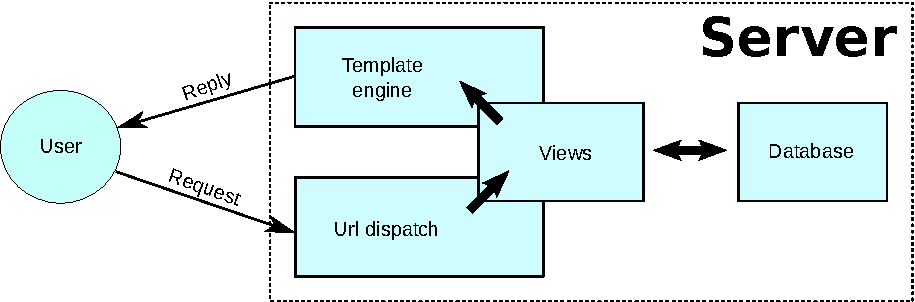
\includegraphics[scale=0.8]{imgs/mvc.pdf}
  \caption{Description du traitement d'une requête d'un client, analysée par
           le résolveur d'URL, traitée par la \textit{view} avec le support
           d'une base de données puis affichée par le moteur de rendu}
  \label{fig:mvc}
\end{figure}

Afin de compléter cette section, il est important d'aborder les \textit{generic view}.
Une vue générique est une fonction fournie par la bibliothèque Django permettant
d'exécuter des actions simples, "que tout le monde fait". Comme par exemple, pour lister
un sous-ensemble d'un type d'objet. Dans
le cas d'une liste de documents relatifs à un cours en particulier, il n'est plus nécessaire que le développeur
écrive une vue particulière car il peut juste référencer la vue
générique dans le résolveur d'URL et donner le nom du template à employer
ainsi que quelques paramètres. Ce projet emploie énormément cette méthode. 

Afin de faciliter la manipulation d'un projet Django, ce dernier fournit un script
de contrôle : le \textit{manager.py}. Ce dernier permet de manipuler la base de
données, créer un \textit{shell} dans l'application, d'exécuter un serveur
web de développement... Les principales commandes sont listées plus bas, le
script est accessible avec la commande \texttt{./manage.py <nom de commande>}.

\begin{description}
\item[syncdb] Construit la base de données. Ce mode passe en revue tous les modèles
              disponibles et crée les tables requises. Il ne permet pas de modifier
              une table existante, ce problème sera abordé dans une section ultérieure.
\item[shell] Exécute un \textit{shell} avec les variables d'environnement Django
             correctement réglées. Ce dernier permet de faire des opérations de maintenance
             sur la base de données, aider à l'implémentation du code en fournissant
             un mode interactif d'exécution...
\item[runserver] Exécute un serveur web localement, fournissant un environnement
             de test au développeur. Ce mode n'est absolument pas adapté à un usage en production.
\item[startapp] Crée une nouvelle Django-app (voir section ultérieur) dans le projet.
\item[test] Lance la suite de tests des applications Django.
\end{description}


\section{Interaction avec la base de données}

Un \textit{Object-relational mapping} (ORM) est une technique
de conversion d'objets en mémoire en enregistrement dans une base de données
relationnelle et inversement. Cette technique est très puissante et permet
au programmeur de ne plus interagir directement avec la base de données, juste
de manipuler des objets. A ce titre, Django possède un ORM, dont les principales
caractéristiquez vont être développées ici.

Comme évoqué dans la section précédente, la fonction \textit{view} a la responsabilité
du calcul de la page. Souvent cette dernière se base sur des informations présentes
en base de données. Chaque enregistrement de cette dernière, pour être exploitable
par Django, devra être assortie à un modèle, c'est-à-dire une \textit{class} Python
ayant une structure compréhensible par Django. Ce dernier créera le type dans la
base de données, y insérera les nouveaux éléments, supprimera ceux qu'il faut...

Par exemple, dans le cadre de l'application de collaboration, il faudra un objet
\textit{cours}. Ce dernier représentera un cours, aura un nom, une description,
un mnémonique (slug\footnote{https://en.wikipedia.org/wiki/Slug\_\%28publishing\%29}).
De plus, il sera possible de lier des documents et des fils de discussion à des
cours, d'où les relations \textit{manytomany} vers des objets de type Document
et Thread.

\begin{verbatim}
class Course(models.Model):
    slug = models.SlugField(unique=True)
    name = models.TextField()
    description = models.TextField(null=True)
    documents = models.ManyToManyField(Document)
    threads = models.ManyToManyField(Thread)
\end{verbatim}

L'ORM de Django permet de manipuler des objets \textit{cours} grâce à une API simple.
Il est possible de créer des nouveaux objets en les instanciant, de les
sauver en base de données, de lire ou modifier une valeur d'un champ,
de les supprimer, comme le monde l'exemple suivant :

\begin{verbatim}
>>> from application.models import Course
>>> c = Course(name="Informatique", slug="info-f-101", description="example")
>>> c
<Course: Informatique>
>>> c.save()
>>> c.name = "Informatique update"
>>> c.name
"Informatique update"
>>> c.save()
\end{verbatim}


\section{Synchronisation entre les modèles et la base de données}

Comme évoqué précédemment, le code décrivant les
modèles est notamment utilisé pour associer les champs des enregistrements
aux propriétés des objets. Cette technique permet de s'occuper des objets uniquement au lieu 
d'interagir avec la base de données.
Au fil de l'évolution du projet, la structure des différents modèles
est amenée à changer : il faut que la structure de la base de données évolue simultanément.
De cette constatation découle plusieurs questions : comment, quoi, qui?

Ce travail conseille d'employer l'application \textit{Django-south}
\footnote{http://south.aeracode.org/}. Cette dernière permet de garder l'état d'un modèle
à différents moments de son développement et à calculer des \textit{deltas} de modèle, équivalent
à un delta d'un code source dans un système de gestion de versions. Ensuite,
à la demande de l'utilisateur, \textit{django-south} applique les \textit{deltas}
(appelées migrations) sur la base de données. Il possède des mécanismes pour les
appliquer dans l'ordre, ne pas les appliquer plusieurs fois, migrer les
données en même temps que le réglage de la table, possibilité de faire un rollback
sur une migration...

Physiquement, les migrations sont stockées dans des fichiers dans un sous-dossier
\textit{migrations} de l'application Django. Elle sont sous la forme de fichier
Python, pouvant être controlées avec un système de gestion de versions. Une explication
détaillée est disponible sur le site de \textit{djangopro}
\footnote{http://www.djangopro.com/2011/01/django-database-migration-tool-south-explained/}.

Par exemple, voici une session d'utilisation de l'outil \textit{Django-south}.
Le scénario d'utilisation est le suivant : sur un ordinateur \texttt{(ve)}, le développeur
ajoute un nouveau modèle \textit{lapin} à l'application \textit{animal}. Ensuite,
il modifie ce modèle en ajoutant un champ. Par la suite, il copie les différents
fichiers sur une autre machine possédant déjà une base de données. Il convient de
modifier cette dernière afin d'être synchronisé avec les sources de l'application,
avec la commande \texttt{migrate}.

\begin{Verbatim}
\textcolor{Blue}{# Django app "animal", un seul modèle : le Lapin, possédant un nom}
(ve) $ cat animal/models.py
from django.db import models

class Lapin(models.Model):
    name = models.TextField()

\textcolor{Blue}{# Initialisation du système Django-south}
(ve) $ ./manage.py schemamigration animal --init
Creating migrations directory at '/home/hastake/mouh/mouh/animal/migrations'...
Creating __init__.py in '/home/hastake/mouh/mouh/animal/migrations'...
 + Added model animal.Lapin
Created 0001_initial.py.
You can now apply this migration with: ./manage.py migrate animal

\textcolor{Blue}{# Application de la migration, contenant le nouveau modèle}
(ve) $ ./manage.py migrate animal
Running migrations for animal:
 - Migrating forwards to 0001_initial.
 > animal:0001_initial
 - Loading initial data for animal.
Installed 0 object(s) from 0 fixture(s)

\textcolor{Blue}{# Modification du modèle, ajout d'un champ, la race du lapin}
(ve) $ cat animal/models.py
from django.db import models

class Lapin(models.Model):
    name = models.TextField()
    race = models.TextField(default="blanc")

\textcolor{Blue}{# Création d'une nouvelle migration ajoutant la race du lapin, application}
(ve) $ ./manage.py schemamigration animal --auto
 + Added field race on animal.Lapin
Created 0002_auto__add_field_lapin_race.py.
You can now apply this migration with: ./manage.py migrate animal
(ve) $ ./manage.py migrate animal
Running migrations for animal:
 - Migrating forwards to 0002_auto__add_field_lapin_race.
 > animal:0002_auto__add_field_lapin_race
 - Loading initial data for animal.
Installed 0 object(s) from 0 fixture(s)

\textcolor{Blue}{# Sur une autre machine, après avoir mis à jour les sources}
\textcolor{Blue}{# de l'application (dont les migrations) : commande "migrate"}
\textcolor{Blue}{# exécute toutes les migrations manquantes}
(ve remote) $ ./manage.py migrate
Running migrations for animal:
 - Migrating forwards to 0002_auto__add_field_lapin_race.
 > animal:0001_initial
 > animal:0002_auto__add_field_lapin_race
 - Loading initial data for animal.
Installed 0 object(s) from 0 fixture(s)

\textcolor{Blue}{# Affichage des migrations :}
(ve) $ ls animal/migrations/
0001_initial.py
0002_auto__add_field_lapin_race.py
__init__.py
\end{Verbatim}

Comme signalé ci-avant, il est indispensable pour un tel projet d'évoluer, c'est pourquoi à
l'heure où ces lignes sont écrites, un nouveau système est déployé sur
les nouvelles versions de Django : \textit{Schema alteration}
\footnote{http://www.kickstarter.com/projects/andrewgodwin/schema-migrations-for-django}
\footnote{https://github.com/django/django/pull/376}. Ce système permet
une plus grande flexibilité, est intégré à Django lui-même, possède un
format de migration beaucoup plus lisible, plus facile à rebaser ou à
fusionner avec d'autres branches et détecte plus de modifications de modèle
automatiquement.


\section{Déploiment d'un projet Django}

Outre Django, une application web a généralement d'autres dépendances. Par exemple
ce travail dépend aussi de l'application \textit{Django-south} détaillée plus haut.
Plus précisément, l'application web dépend de logiciel externe ayant certaines versions.
Par exemple, un site fonctionnant sous Django 1.4 aura besoin de quelques modifications
pour fonctionner sous Django 1.5 et ne fonctionnera probablement pas du tout sous
Django 1.6. Pour éviter au développeur de s'arracher les cheveux, l'écosystème Python
fournit un outil, nommé \textit{virtualenv}.

Un environnement virtuel (\textit{virtualenv}) est une sandbox
\footnote{https://fr.wikipedia.org/wiki/Sandbox\_\%28s\%C3\%A9curit\%C3\%A9\_informatique\%29}
permettant d'installer toute une série de bibliothèques pour l'environnement
local sans perturber le système hôte. Cela permet d'avoir l'ensemble des dépendances
logiciels à une version prédéfinie localement.

Pour distribuer et installer facilement une bibliothèque, l'écosystème Python
possède un logiciel nommé \textit{pip}. Ce dernier se base sur le
\textit{Python Package Index} (PyPi), un répertoire de plusieurs centaines de
paquets Python, disponible à l'installation, avec un système de dépendance.
Pour automatiser l'installation, il est d'usage d'écrire un fichier, conventionnellement
nommé \textit{requirement.txt}, listant les dépendances de l'application.

Par exemple, dans le cas de la plateforme, voici la méthode pour travailler avec  l'environnement
virtuel et l'installateur de dépendances :

\begin{Verbatim}
\color{Blue}{# Liste des dépendances du projet}
$ cat requirements.txt
django
pypdf
south
markdown

\color{Blue}{# Création d'un nouvel environnement virtuel}
$ virtualenv --distribute --no-site-packages ve
New python executable in ve/bin/python2.7
Also creating executable in ve/bin/python
Installing distribute. done.
Installing pip. done.

\color{Blue}{# Activation de l'environnement virtuel}
\color{Blue}{# Cette commande est à exécuter chaque fois que l'utilisateur veut l'utiliser}
$ source ve/bin/activate

\color{Blue}{# Installation des dépendances}
(ve) $ pip install -r requirements.txt
\end{Verbatim}


\section{Description des fonctionnalités}

La plateforme web est construite autour d'un petit nombre de pages web, chacune
ayant un rôle fonctionnel. Cette section décrit ces dernières.

Après authentification l'utilisateur voit la page d'accueil. La première fois qu'il
utilise le système, un message d'aide est affiché, il peut le masquer par la suite.
Il est invité à sélectionner des cours grâce au menu de la barre de navigation,
qu'il peut choisir de suivre. Les cours suivis sont repris sur la page d'accueil, ainsi
que quelques statistiques à propos de ses cours, comme la dernière activité y relative.
La figure \ref{fig:home} présente la disposition générale de cette page.

Le scénario classique d'utilisation de la plateforme consiste à sélectionner un cours
et regarder les ressources disponibles pour ce dernier. Cette page est présentée en
figure \ref{fig:course}. Cette page permet à l'utilisateur de voir une liste de documents
jugé intéressants pour ce cours ainsi qu'une liste de fils de discussion liée à ce cours.
C'est aussi sur cette page qu'il peut décider de suivre ou d'arrêter de suivre un cours.
Via cette page, l'étudiant peut uploader un nouveau document, voter pour les documents
qu'il juge intéressants ou les fils de discussion importants.

S'il choisit de cliquer sur un document, une visionneuse de document lui est proposée.
Cette page, présentée en figure \ref{fig:viewer}, affiche le rendu de chaque page
du document PDF ainsi qu'une liste de miniatures pour faciliter la navigation. Il
est possible de zoomer et de télécharger le document à partir de cette page. En
dessous de chaque page du document PDF, ainsi que sur l'ensemble du document, il
est possible de laisser un commentaire, pour initier un nouveau fil de discussion.

Ces différents commentaires sont tous affichables avec la page forum. Chaque page
est une suite de commentaires, par différents auteurs, auquel il est possible
de répondre. Chaque fils de discussion est lié à une ressource, un cours, un
document ou à une page d'un document. Par exemple, si la page 2 d'un document
est commenté, le fil de discussion apparaitra dans les fils de discussion
relatifs à la page, au document et au cours. Par contre, si l'utilisateur
poste un commentaire relatif à tout le cours, il ne sera listé que sur la page
du cours. Il est possible de mettre en page les différents commentaires avec la syntaxe
\textit{markdown}, une approche très populaire sur internet.

Outre ces fonctions principales, le site possède un \textit{wall}, un mur
de notification. Lorsqu'un évènement se produit, c'est-à-dire
si quelqu'un uploade un nouveau document, poste un nouveau commentaire ou répond
dans un fil de discussion, une notification est ajoutée au mur. Ce mur possède
une page RSS qu'il est possible d'ajouter à son lecteur de flux préféré.

De plus, le site contient une fonction recherche de document (détaillée dans une
section ultérieure), une interface administrateur qui permet d'éditer les permissions
des utilisateurs, la structure des catégories et des cours et de gérer les documents.
Finalement, deux forums sont mis à la disposition des étudiants pour poster
des commentaires relatifs aux problèmes qu'ils rencontrent ou pour faire des suggestions.

\begin{figure}
  \centering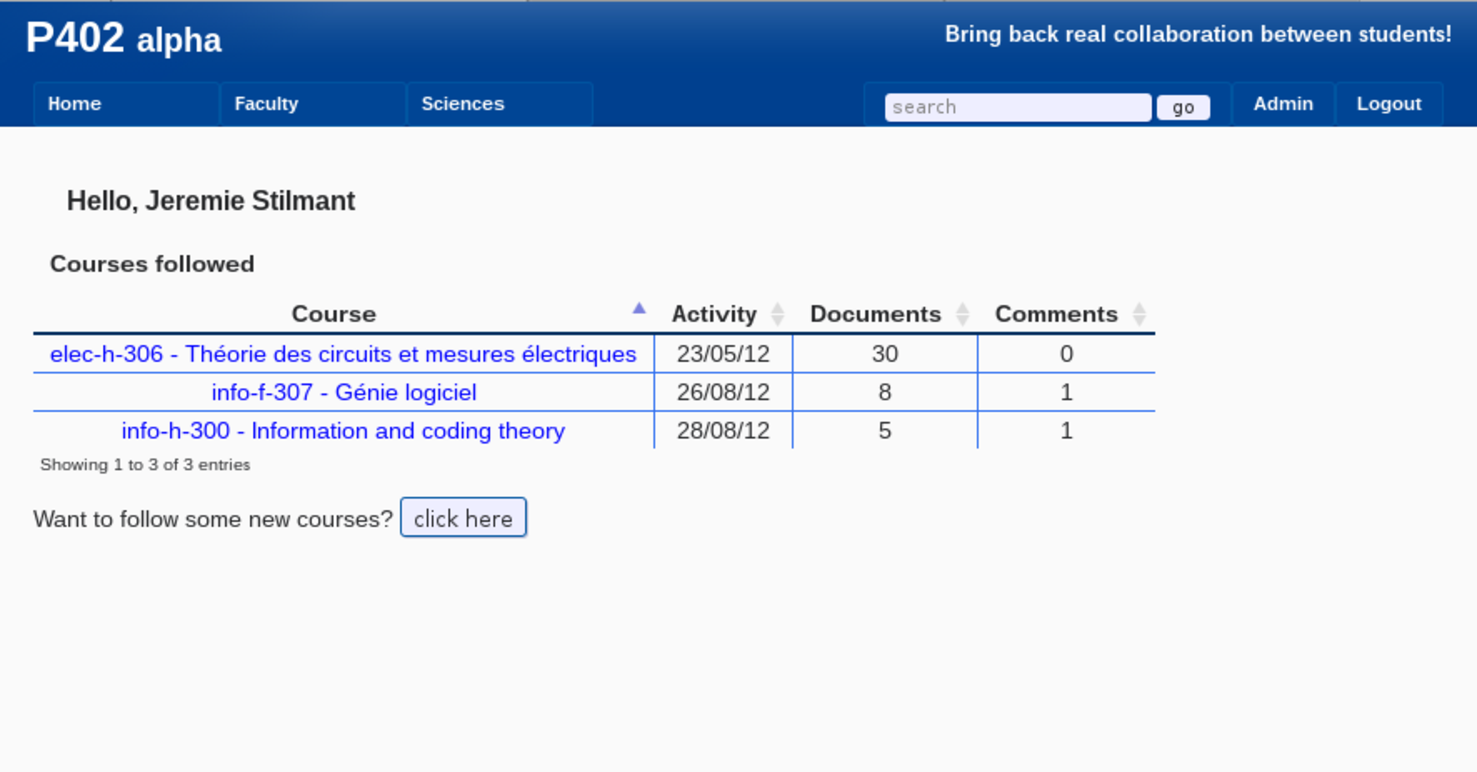
\includegraphics[scale=0.5]{imgs/home.pdf}
  \caption{Page d'accueil d'un étudiant suivant 3 cours sur le site}
  \label{fig:home}
\end{figure}

\begin{figure}
  \centering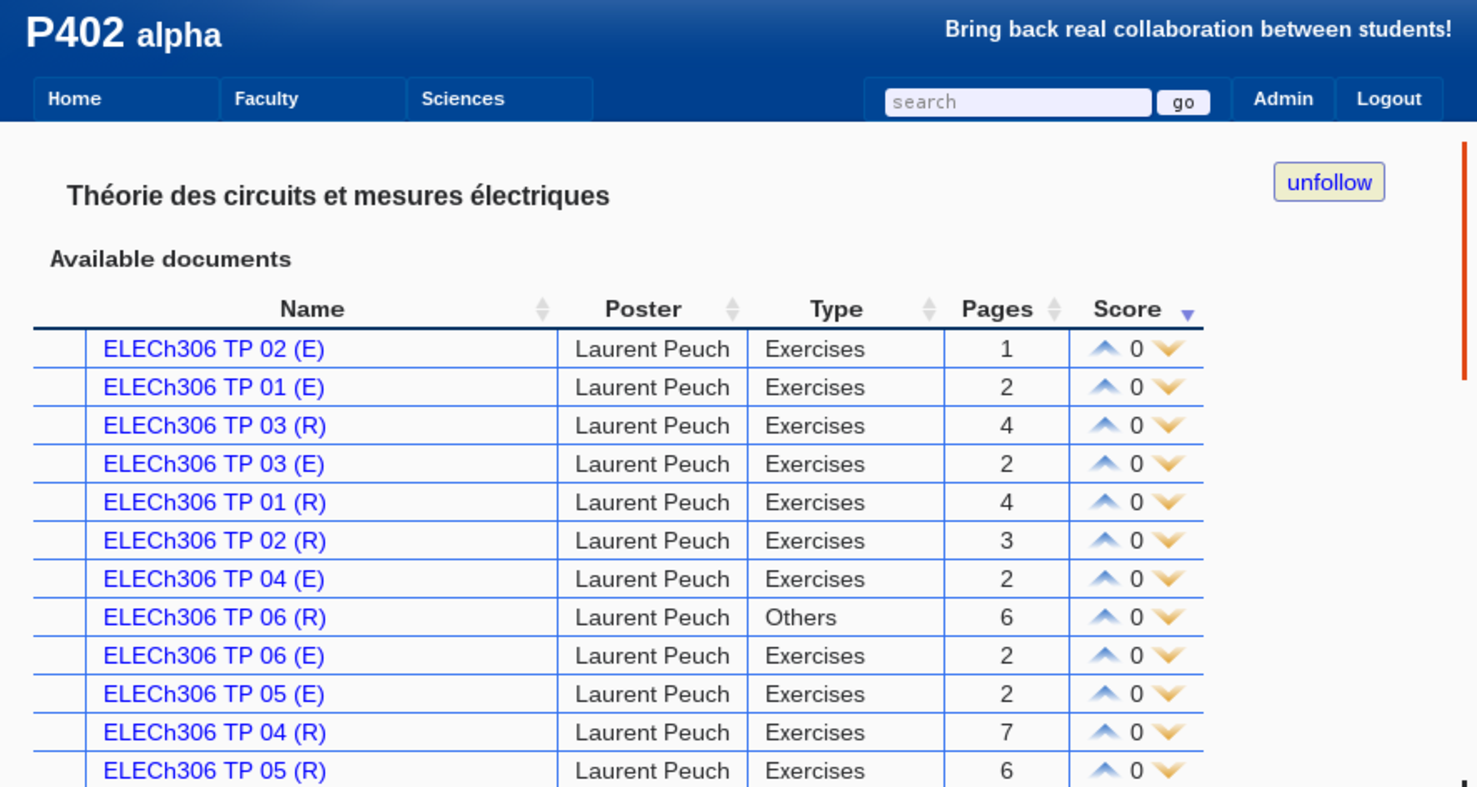
\includegraphics[scale=0.5]{imgs/cours.pdf}
  \caption{Page de cours des circuits et mesures électroniques}
  \label{fig:course}
\end{figure}

\begin{figure}
  \centering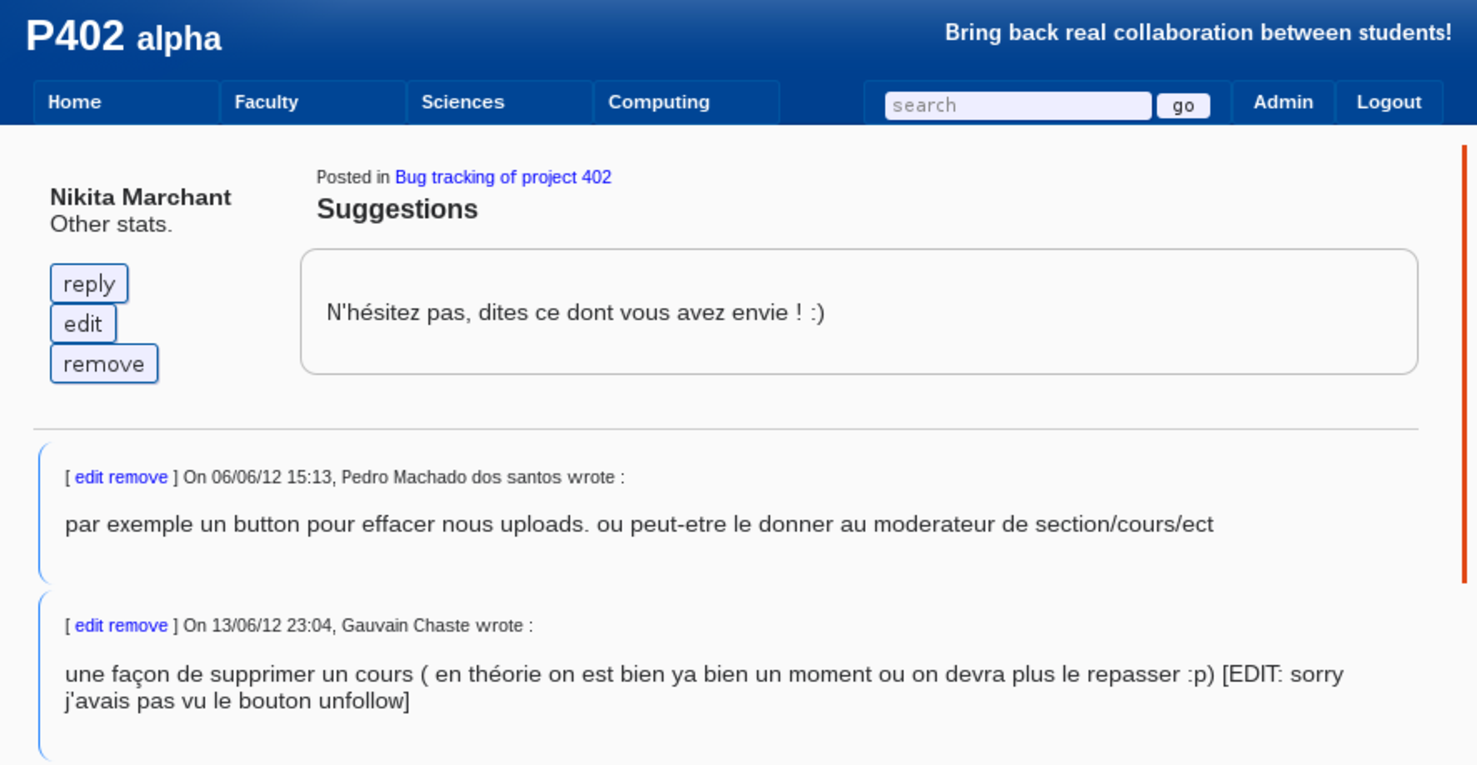
\includegraphics[scale=0.5]{imgs/forum.pdf}
  \caption{Fil d'un forum de discussion}
  \label{fig:forum}
\end{figure}

\begin{figure}
  \centering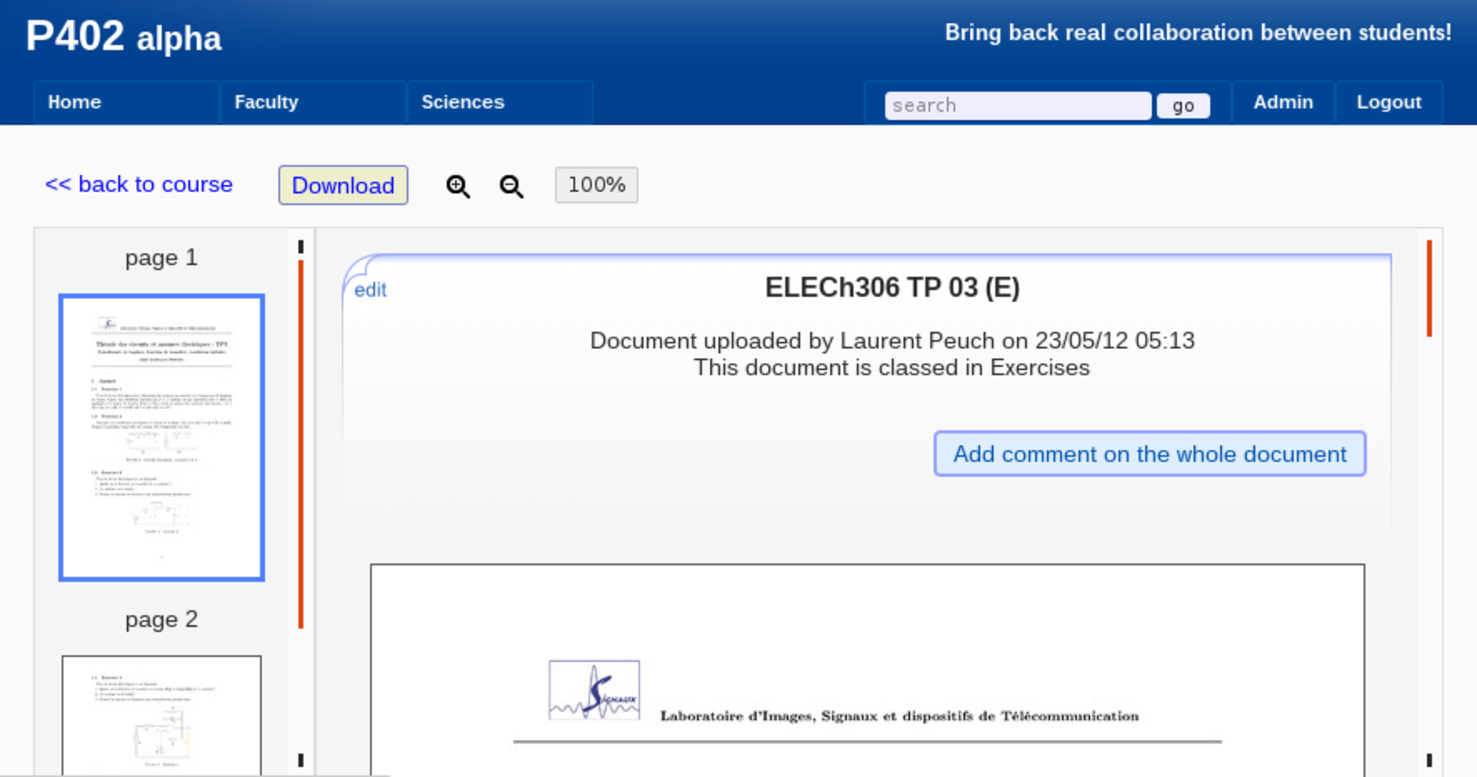
\includegraphics[scale=0.5]{imgs/viewer.pdf}
  \caption{Visionneuse de document PDF, affichant un TP d'électronique}
  \label{fig:viewer}
\end{figure}
	
\begin{figure}
  \centering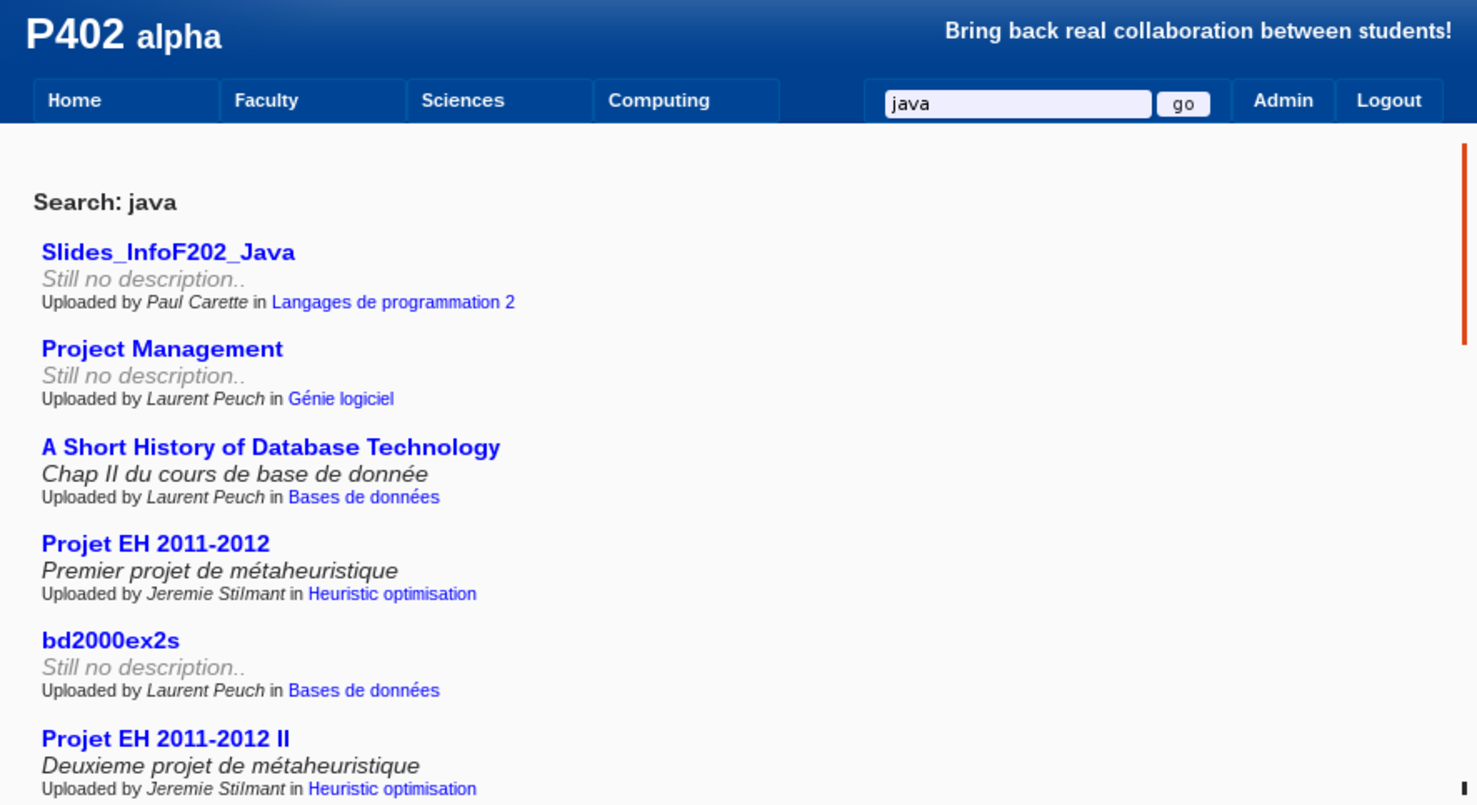
\includegraphics[scale=0.5]{imgs/search.pdf}
  \caption{Fonction recherche avec comme mot clé \textit{java}}
  \label{fig:search}
\end{figure}


\section{Architecture des différents composants}

Le projet est découpé en différents
composants, détaillés dans cette section. Cette modularité permet de prendre en main le projet plus facilement
et de simplifier la maintenance. De plus, il oblige le développeur à
prendre en compte le couplage entre les différents composants, ce qui mène
à des logiciels moins complexes.

Dans l'univers Django, une Django-app est un module Python contenant des
ressources, comme les modèles de ce module, les views, la manière de reconnaitre
une URL, les templates associés... Chaque module possède la même structure : un fichier
\texttt{\_\_init\_\_.py} pour indiquer que c'est un module, les fichiers
\texttt{views.py, models.py} et \texttt{urls.py} pour le fonctionnement du module,
un fichier optionnel \texttt{test.py} contenant les tests du module, un dossier
\textit{templates} contenant les fichiers HTML et parfois un dossier \textit{migrations}
pour la synchronisation avec la base de données.

Chaque application Django est responsable d'une famille de fonctionnalités du site.
Généralement ces familles sont construites autour d'un type d'objet. L'application
représente les cours sous forme de hiérarchie : les cours sont agrégés en catégories,
ces dernières sont elles-mêmes inclues dans d'autres catégories, de manière récursive,
jusqu'à une catégorie nommée "Root". Les cours et les catégories sont donc
placées dans un arbre. Chaque cours ou catégorie peut être inclu dans plusieurs
autres catégorie en même temps : par exemple un cours peut être référencé dans
une catégorie lié à la partie Polytechnique de l'arbre et dans une catégorie liée à la
partie Informatique.

Généralement, l'arbre est divisé selon la même structure que l'université : faculté,
section, année, options. Chaque feuille peut contenir des cours ou des sous-catégories.
Chaque cours peut contenir des fils de discussion et des documents. Tous ces
types d'objets sont gérés par les applications suivantes :

\begin{description}
\item[admin] Application fournissant trois outils d'administration : la gestion
   des utilisateurs et des permissions, la gestion des documents et la gestion
   de l'arbre de catégorie et cours. Ces outils permettent de supprimer des éléments,
   les modifier et parfois d'en créer.
\item[catégories] Application fournissant le support de l'objet catégorie :
   des fonctions pour les créer, éditer, supprimer ainsi que les attacher/détacher de l'arbre
\item[courses] Application fournissant le support de l'objet cours :
   des fonctions pour les créer, les modifier et les manipuler (par exemple compter le nombre
   de documents ou fils de discussion qu'ils contiennent)
\item[documents] Application contenant les objets document et page, permettant de les
   créer et manipuler. Cette application inclut aussi un ensemble de fonctions pour
   voter sur les documents, les télécharger et les uploader, les lister suivant certains
   paramètre... L'application contient aussi le processus de traitement des documents
\item[messages] Application contenant les objets fil de discussion et post, les méthodes
   pour les manipuler (création, édition, suppression, vote)
\item[notifications] Application gérant le système de création d'évènements. Il existe
   un objet par type d'évènements mais ces derniers sont tous stockés dans la même
   table grâce à un système basé sur des métaclasses. Il existe 4 types d'évènements :
   \textit{Annoucement, ReplyEvent, ThreadEvent} et \textit{UploadEvent}. L'application
   contient aussi le mur de notification et le flux RSS
\item[search] Application permettant la recherche dans le corpus de document
\item[upvotes] Application gérant le système de vote des documents et des fils de discussion.
   Cette application permet de classer les documents et fils par type à chaque vote
   (par exemple pour un document, il est possible que le public change son classement
   de "projet" à "ancien projet" avec assez de vote). Elle garde aussi un historique
   du vote de l'utilisateur afin d'éviter les doublons.
\item[users] Application gérant le profil d'un utilisateur, les cours qu'il suit, le
   message d'accueil. Elle s'occupe aussi de déterminer si l'utilisateur a les permissions requises.
\end{description}


\section{Configuration de la plateforme}

Un projet Django se configure via un fichier nommé \textit{settings.py},
présent dans le dossier racine. Ce fichier est au format Python et est principalement
une suite de définition de variables. Cette section cherche à détailler la majorité
de celles utiles pour le projet.

\begin{description}
\item[Debug, Debug\_template] Ces variables, de type booléennes, permettent d'activer
      ou d'inhiber l'affichage de commentaires et d'information lorsqu'une erreur
      intervient sur le site.
\item[Database] Cette variable stocke les informations sur la base de données. Elle
      permet de spécifier la bibliothèque à employer (sqlite3 pour le développement
      et postgresql\_psycopg2 pour la production), le nom de la base de données, l'utilisateur
      et le mot de passe à employer.
\item[Upload\_log] Variable contenant un chemin absolu vers l'endroit où logger
      les informations du gestionnaire d'upload de document.
\item[Installed\_app] Ce tuple liste toutes les applications Django à employer. Il
      doit contenir toutes les applications internes de Django à activer (par exemple
      le système de session), les applications de partie tiers hors Django (par exemple
      \textit{south}) ainsi que toutes les applications développées pour la plateforme,
      détaillées dans la section précédente.
\item[Template\_dirs] Ce tuple doit contenir tous les chemins d'accès au dossier
      contenant des \textit{templates} qui ne sont pas liés à des applications Django.
\item[Root\_urlconf] Chaine de caractères indiquant le fichier à employer comme
      base pour le résolveur d'URL
\item[Static\_root, Static\_url] Chaines de caractères contenant les informations
      pour la livraison des fichiers statiques aux clients
\item[Convert\_pdf] Variable booléenne indiquant si la conversion PDF est active
\item[User\_check] Chaîne de caractères référençant l'URL à employer pour contacter
      le système d'authentification de l'ULB
\item[Upload\_dir] Chaîne de caractères indiquant le chemin vers le dossier contenant
      les pdf, leurs pages...
\item[Parsing\_worker] Nombre de traitements de PDF maximum en parallèle
\end{description}


\section{Traduction du site}

Afin d'être accessible à un maximum d'étudiants, la plateforme étudiante est actuellement traduite
en deux langues : anglais et français.
Cette étape est rendue simple par Django qui supporte par défaut les systèmes
de localisation\footnote{https://docs.djangoproject.com/en/dev/topics/i18n/translation/}.

Pour traduire la plateforme, la première étape a été de marquer les chaines de
caractères affichées au client. Grâce à la séparation entre le contenu et la présentation,
tous les textes affichés aux clients sont dans les \textit{templates}. Cette concentration
a permis de gagner beaucoup de temps.

Pour déclarer un texte à traduire, dans un \textit{template}, il y a deux manières
de procéder. Si le texte est court, il peut être affiché grâce à la commande 
\texttt{\{\% trans "du text" \%\}}. Par contre, si le texte est plus long, inclut des
éléments HTML ou plus, il faut employer une déclaration par block, intercalée entre
deux commandes : \texttt{\{\% blocktrans \%\}} et \texttt{\{\% endblocktrans \%\}}.
Un exemple est disponible ci-dessous.

\begin{verbatim}
<h1>{{ username}}</h1>


<p>Welcome in this <strong>strange</strong> place.</p>

\end{verbatim}

Grâce à ces marqueurs, Django connait exactement ce qu'il faut traduire dans le site.
Malheureusement, à ce stade il ne ignore comment le traduire. Dans ce cas-là,
par défaut, il va afficher le texte d'origine. Django utilise l'utilitaire GNU
standard \textit{gettext} pour la traduction.

La seconde étape est d'extraire toutes les chaines de caractères
marquées dans un fichier de messages (ayant l'extension \textit{.po}).
Pour ce faire, la commande suivante du
manager est à exécuter : \texttt{django-admin.py makemessages -l fr}. Cette commande
regroupe toutes les traductions d'une langue et fournit à Django une association
entre les chaînes d'origines et les chaînes traduites. Il importe alors que le traducteur
complète ce fichier. Une fois cette étape effectuée, le fichier de traduction 
doit être compilé au moyen de la commande \texttt{django-admin.py compilemessages}.
Cette opération doit être réitérée à chaque modification du fichier de traduction.

Pour que le site puisse fournir au client la langue de son choix, il faut inclure
un sélecteur de langue. Par exemple, dans un \textit{template}, il suffira d'ajouter
le formulaire suivant : 

\begin{verbatim}
<form action="/i18n/setlang/" method="post">
  
  <input name="next" type="hidden" value="{{ redirect_to }}" />
    <select name="language">
      
      
      <option value="{{ language.code }}">
        {{ language.name_local }} ({{ language.code }})
      </option>
      
    </select>
    <input type="submit" value="Go" />
</form>
\end{verbatim}


\section{Traitement des documents}

Une fonction utile pour le projet est de fournir aux étudiants la possibilité
de visionner un PDF directement dans l'interface web au lieu de les obliger
à le télécharger. Cette fonction est similaire à la visionneuse de documents fournie
par Google Doc. Pour offrir ce service, il est impossible de calculer le rendu du PDF
à chaque fois que l'étudiant charge la visionneuse, il faut donc prétraiter chaque
document lors de l'upload. Cette section couvre l'architecture du \textit{processing-daemon},
une application parallèle au serveur web qui se charge de cette tâche.

Le traitement d'un PDF est très lourd, dans le cadre de ce projet il est déjà
arrivé que cette application passe plusieurs dizaines de minutes et emploie des centaines
de mégabytes de RAM pour traiter un document de plus de 200 pages. Il faut
donc que cette application puisse lancer un traitement dès qu'un document arrive
mais ne pas lancer trop de traitement en parallèle : un mécanisme asynchrone est requis.
Pour l'implémenter, il a été décidé de doter le modèle d'un document d'une propriété,
le statut, pour indiquer où en est le traitement. Trois statut différents existent :  \textit{pending}, c'est-à-dire
que l'utilisateur vient de l'uploader mais que le traitement n'a pas encore commencé,
\textit{inprocess}, c'est-à-dire en cours de traitement et \textit{done} quand il est terminé.

Afin d'accélérer le processus, il est possible de spécifier un certain
nombre de traitements réalisables en parallèle : la boucle principale du \textit{processing-daemon}
est donc une série de \texttt{fork} et de \texttt{wait} : chaque enfant pourra exécuter un traitement.
Toutes les 10 secondes, le \textit{processing-daemon} va exécuter une requête à la base
de données pour savoir combien de documents il y a à traiter. S'il y en a, il va les confier
à ses enfants, dans la limite disponible, et modifier le statut du document.

Le rôle principal de chaque enfant est d'extraire de chaque document une série
d'images représentant les pages. Comme l'indique la capture d'écran de la figure \ref{fig:viewer},
il y a deux types d'images : les miniatures (180px de large) et la page au zoom 
choisie par l'utilisateur. Malheureusement, le zoom utilisateur est calculé par
le navigateur à partir d'un rendu : généralement, il n'est pas très bon, et plus il
est éloigné de la résolution d'origine, moins il est bon. Pour chaque page, en
plus de la miniature, le \textit{processing-daemon} va extraire plusieurs "grandes"
images qu'il emploiera au mieux, en fonction du zoom utilisateur courant.

En plus de l'extraction d'images, le \textit{processing-daemon} extrait les mots
du PDF pour la fonction recherche (voir section sur la fonction recherche) ainsi que
plusieurs statistiques comme la hauteur de chaque page, le nombre de pages...


\section{Fonction de recherche}

Actuellement, le projet héberge plusieurs centaines de documents (1440 à l'heure où ces lignes sont écrites).
Afin de permettre à l'utilisateur de trouver un document particulier, une
fonction de recherche fut implémentée. Tout d'abord, cette section abordera
la question de précalcul sur les documents présents, exécutée lors
du traitement d'un document lors de son upload. Ensuite, cette section
détaillera la fonction de calcul du classement des documents en fonction
d'une certaine requête.

Le traitement des documents évoqué à la section précédente inclut une extraction
textuelle. Au moyen de la bibliothèque \textit{poppler}, il transforme un document
PDF en une représentation textuelle. Ensuite il extrait les mots de cette représentation
puis leur racine morphologique grâce à un processus appelé \textit{stemming}
\footnote{https://en.wikipedia.org/wiki/Stemming}. Enfin, pour tout document,
il compte le nombre d'occurrences de chaque racine ainsi que le nombre total de mots du document.
Il sauvegarde l'ensemble de ces informations dans une base de données (le tuple : document, racine, nombre).

Le \textit{term frequency–inverse document frequency} (TF-IDF) est un indicateur
qui reflète l'importance d'un mot dans un document par rapport à son importance
dans l'ensemble du corpus de document. Il est proportionnel à la fréquence d'un terme
d'un document par rapport à la fréquence de ce terme dans l'ensemble des documents.
Par exemple, le verbe "être" est très fréquent dans tous les documents, il aura
un très faible TF-IDF, probablement constant pour tous les documents,
alors que le nom "sécurité" aura un TF-IDF beaucoup plus élevé dans un document
relatif à la sécurité informatique (parce que le terme sera souvent employé)
par rapport à un document sur les mathématiques discrètes (où il ne sera probablement
pas présent). Cet indicateur est la première manière utilisée pour classer
un document par rapport à un autre étant donné une requête de recherche.

Il est intuitif de se dire que les documents souvent visités sont
plus importants. Le classement brut fourni par le calcul du TF-IDF est donc raffiné
par rapport au nombre de vues et téléchargements des documents.

Par exemple, avec le terme \textit{java}, la recherche trouve des documents de langage
de programmation, base de données, informatique fondamentale, etc, comme le montre la figure
\ref{fig:search}.


\section{Authentification des utilisateurs}

Une spécification du projet était de pouvoir garantir que seuls les étudiants de l'ULB
pouvaient accéder aux ressources offertes par ce site, principalement pour des raisons
de propriété intellectuelle et parce que certains professeur sont réticents à 
ce que des éléments extérieurs puissent télécharger des cours. De plus, afin
de ne pas pousser les étudiants à s'autocensurer, il a été décidé que seuls ces derniers
pourraient employer les forums de discussion, sans interférence extérieure.

Dans ce cadre, une réflexion sur la manière d'authentifier les étudiants
a été lancée. Pousser les étudiants à devoir s'inscrire sur le site, en faisant des
vérifications sur leur identité était un mécanisme couteux, c'est pourquoi il a été décidé
d'employer le système d'authentification de l'ULB. Ce système a comme avantages :
\begin{itemize}
\item l'utilisateur n'a pas besoin d'un login et mot de passe supplémentaire
\item le système connait avec précision si l'étudiant est ou non de l'ULB
\item le système possède des informations comme la section de l'étudiant ou
      l'année dans laquelle il étudie.
\item le système ne prend pas de responsabilité au niveau de stockage de mot de passe
\end{itemize}

Cette approche présente aussi deux défauts majeurs : il est dépendant du système
d'authentification de l'ULB. si celui-ci est en panne, les étudiants ne peuvent plus
accéder au site. Ensuite, il est très difficile de faire des exceptions à ce comportement,
par exemple pour des étudiants ayant des problèmes d'inscription? les ressources
sont indisponibles tant que le service inscription n'a pas réglé le problème.

En pratique, le système d'authentification est relativement simple. Comme le montre
le diagramme en figure \ref{fig:auth}, une fois que le client a demandé une
authentification au site de partage de cours, il est redirigé vers la page d'authentification
de l'intranet de l'ULB. Ce dernier fournit un formulaire classique de demande de
NetID et de mot de passe. S'il est valide et que l'utilisateur a le droit d'employer
l'application (s'il est étudiant), il est redirigé vers la page d'authentification
interne du projet, avec deux paramètres : UID et SID. L'\textit{user ID} (UID) est
un identifiant d'utilisateur et le \textit{session ID} est l'identifiant de session.
Ces deux paramètres sont transmis à la plateforme, par le client, via la redirection de l'authentificateur
de l'ULB. Ces paramètres vont être utilisés par la plateforme pour faire
une requête à l'authentificateur de l'ULB pour en vérifier la validité et télécharger
les informations liées à cet utilisateur. Une fois validé, la page index est présentée à
l'utilisateur.

\begin{figure}
  \centering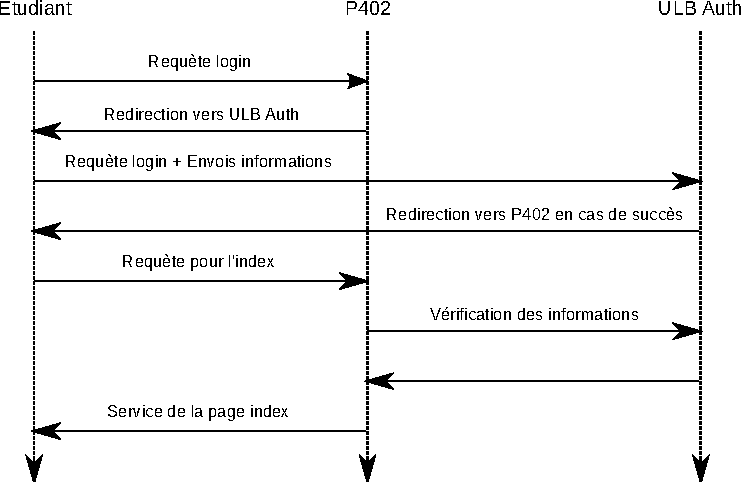
\includegraphics[scale=0.9]{imgs/auth.pdf}
  \caption{Diagramme des connections entre le client, la plateforme et l'authentificateur
de l'ULB lors d'une authentification réussie}
  \label{fig:auth}
\end{figure}

\section{Sécurité de la plateforme}

D'une manière générale, les notions de sécurité sont importantes en informatique
et le domaine du web ne fait pas exception. Une fois déployé en production,
un site web est susceptible de se faire attaquer par n'importe qui, il est donc
important de passer en revue les vulnérabilités les plus populaires et de les prévenir.

Tout d'abord, un premier type de vulnérabilité est le concept de SQL Injection. Cette attaque
consiste à déformer une requète SQL de son but premier dans le but de détourner
le résultat de cette requête. Généralement, les requêtes contiennent le contenu
de variable, parfois venant d'entrée utilisateur et ce dernier peut essayer
de faire "déborder" ces variables pour transformer la sémantique de la requête. Par
exemple, si un algorithme d'authentification cherche à vérifier que l'utilisateur existe
et possède le bon mot de passe, il pourrait exécuter la requête ci-dessous.
Un utilisateur malveillant pourrait entrer une autre valeur et si l'algorithme
vérifie le résultat de retour (0 pour l'utilisateur inexistant, 1 pour l'utilisateur
existant), l'attaquant pourra se logger.	

\begin{Verbatim}
SELECT count(*) FROM users
  WHERE username = "lama" and password = "secret";

SELECT count(*) FROM users
  WHERE username = "\textcolor{Blue}{lama" or 1 = 1 LIMIT 1;#}" and password = "";
\end{Verbatim}

Avec le framework Django, l'ORM est protégé contre les injections SQL à plusieurs
niveaux. D'une part, les valeurs entrées dans les formulaires sont nettoyées avant
d'être employées dans les fonctions \textit{views} et l'ORM possède un mécanisme
de sécurité contre tout type d'injection connue.

Un autre type d'attaque très populaire est le \textit{cross-site scripting} (XSS).
Il s'agit d'insérer dans une page un script malicieux, généralement dans du contenu
produit par l'utilisateur (commentaire sur un forum, nom d'utilisateur sur une page de profil...)
qui va s'exécuter dans le navigateur des autres clients, pouvant voler des informations.

Pour se protéger de cette attaque, Django nettoie les formulaires des entrées utilisateurs
comme évoqué précédemment, ensuite il empêche du contenu de script ou HTML d'être directement
rendu dans la page web au niveau du moteur de \textit{template}. Par exemple,
si le développeur veut afficher le texte d'un commentaire, le template pourrait contenir
\texttt{\{\{ comment \}\}}. Si la variable \textit{comment} contient du HTML,
il sera transformé en texte, sans pouvoir être interprété par le navigateur du client.

Enfin, une attaque courante est le concept de \textit{cross site request forgery} (CSRF).
C'est une attaque un peu plus évoluée que les deux précédentes, impliquant la fabrication
d'une requête HTTP vers le site venant d'un site malveillant. Cette requête est généralement
une requête de type POST, exécutant quelque chose. Si l'utilisateur est loggué sur le site,
cette requête pourrait avoir un réel impact.

Il est trivial de se protéger contre cette attaque. Le formulaire générant la
requête contient un numéro unique et ce numéro est aussi stocké dans un cookie présent
dans le navigateur du client. Seul quelqu'un pouvant lire ou régler ce cookie pourra
fabriquer un formulaire que Django acceptera. Si la sécurité du navigateur du client
est correcte, c'est-à-dire qu'un site tiers ne peut lire ou modifier les cookies d'un
autre site, alors seules les requêtes venant de la plateforme seront acceptées.

De nouvelles attaques sont publiées régulièrement. Un aspect de la sécurité de la plateforme
est aussi de la maintenir à jour, en suivant les publications de nouvelles versions
et de bulletin de vulnérabilité.


\section{Test de la plateforme}

Une partie importante du travail d'un développeur est de s'assurer que l'application
fonctionne correctement. Pour une plateforme web, cette tâche est particulièrement
compliquée. Cette section cherche à couvrir les solutions envisagées dans le cadre
de ce projet.

D'une manière générale, les tests doivent être écrits avec la bibliothèque
\textit{unitest2}. Pour lancer la suite de tests, il faut exécuter la commande
\texttt{./manage.py test}. L'étape la plus compliquée du processus est de créer
une "fausse" base de données, utilisée par tous les tests. Malheureusement, suite
à la mise en production de la plateforme et à l'usage de Django-south, la création de cette
base de données est très compliquée et la suite de tests n'a pas été adaptée au nouveau
schéma de base de données. Ils ne sont pas inclus dans la version de la plateforme
actuellement en production, mais les commentaires de cette section restent cependant
valides.

La technique utilisée pour écrire un test est relativement simple : il faut ajouter une classe
Test par application puis faire une série de méthodes pour chaque aspect testé.
Par exemple, pour l'application utilisateur, il pourrait être utile de vérifier
si la suppression du message d'accueil fonctionne.
Le développeur pourrait employer le test suivant :

\begin{verbatim}
import unittest
from django.test.client import Client

class SimpleTest(unittest.TestCase):
    def test_details(self):
        client = Client()
        response = client.get('/user/mask_welcome/')
        self.assertEqual(response.status_code, 200)
\end{verbatim}

De cette manière, la fonction en question est appelée et le test vérifie qu'elle
retourne un résultat acceptable. Malheureusement, elle ne vérifie pas si elle a fonctionné,
pour cela, il faudrait vérifier si le message est bien masqué. Le développeur pourrait
employer l'assertion \texttt{self.assertNotContains(response, "un morceau du message")}.

Le résultat de la plateforme est une série de page web. Afin de vérifier la constance
dans l'affichage des pages, le développeur pourra être intéressé par l'outil Wraith,
développé par la BBC\footnote{https://github.com/BBC-News/wraith}. Ce dernier
permet de faire un rendu de la page web et le comparer avec les précédentes versions
des rendus, permettant de détecter des changements. C'est intéressant pour les
questions de CSS notamment.


\section{Continuous testing et Github}

Un contrôle de révision de source est un système permettant de garder un historique
de toutes les versions du code source d'un projet. Il permet de partager les ressources
entre différents développeurs, développer les fonctionnalités isolées entre-elles sous
forme de branches, exécuter plusieurs versions du logiciel... Un système de révision
de source distribué est un système de révision sans serveur central. Chaque
utilisateur de ce système possède l'entièreté de l'historique et des informations,
il n'y a pas de source d'autorité sur le code source.

Ce projet a été développé sous Git, un système de révision de source utilisé notamment
pour le kernel Linux. Il est très puissant et très populaire. Afin de publier le code
source, le site Github fut employé.

Git permet aux développeurs de créer des branches. Ces dernières sont une suite de
contributions aux sources (commit) partant d'un état commun. Par défaut, il existe
au moins une branche, nommée \textit{master}, qui est employée dans ce projet
pour symboliser une version prête pour la production.

La méthode de travail employée a été de développer certaines fonctionnalités en branches
distinctes de \textit{master}, de tester ces branches puis de les incorporer dans
le tronc principal. Une fois que ce dernier était mis à jour, il fallait mettre en
place la nouvelle version en production. Pour ce faire, le concept de \textit{git hook}
a été employé : il est possible de générer un signal après certains types d'évènements.
Dans ce cas-ci, après le \textit{push} d'une nouvelle version sur le dossier Github,
le serveur était mis au courant de l'évènement et téléchargeait la nouvelle version (avec
\textit{git pull}).

Afin de pouvoir mettre en production des versions expérimentales, le serveur a été
modifié pour pouvoir créer dynamiquement des \textit{vhosts} (il suffit d'ajouter un
fichier de configuration type dans le dossier \texttt{vhost.enabled} puis de le redémarrer).
Ensuite, à chaque \textit{git push} sur Github, si la chose poussée était une
branche commençant par le texte \texttt{vhost\_}, un nouveau \textit{vhost} était créé avec
le contenu de la branche et une copie de la base de données de production.
De cette manière, la version expérimentale pouvait être essayée avant de la
fusionner avec le tronc commun. Cette approche est détaillée par la figure \ref{fig:git}.
Le \textit{continuous testing} peut être implémenté sur ce mode de fonctionnement : avant
de mettre le site en ligne, le script créant le \textit{vhost} pourrait exécuter la suite
de test et afficher le résultat s'il y a un problème. S'il y en a pas, il affiche
la plateforme.

\begin{figure}
  \centering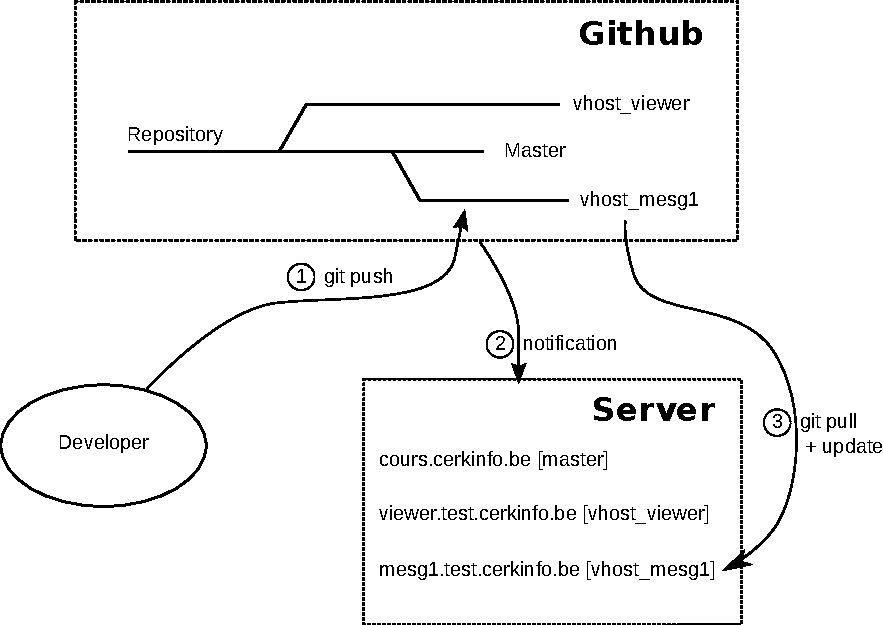
\includegraphics[scale=0.9]{imgs/git.pdf}
  \caption{Diagramme présentant l'approche employée pour développer par fonctionnalités
           et faire des tests proches de l'environnement de production}
  \label{fig:git}
\end{figure}


\section{Conclusion}

Ce document présente globalement la plateforme étudiante déployée dans le cadre de ce projet sur le serveur du
Cercle Informatique. L'idéal recherché au travers de cette plateforme est la mise en place d'un service 
faciliant le partage par les étudiants de documents relatifs aux cours.

Cette plateforme a rencontré un réel engouement et au niveau du partage il s'agit d'un franc succès 
puisqu'elle a été employée par plus de 600 étudiants depuis sa mise en service en mai 2012.
A ce jour, plus de 1400 documents sont hebergés sur la plateforme,
ils sont par conséquent consultables en ligne ou téléchargeables.

Au vu de la demande du corps académique, l'accès à la plateforme a été restreint à la communauté des étudiants 
de l'ULB. 
Grâce son authentification basée sur le NetID de l'ULB, elle est accessible à tous les étudiants,
bien que pour l'instant les seuls cours intégrés sur la plateforme soient
les cours d'informatique, de physique et de math de la faculté des sciences ainsi
que l'ensemble des cours de premier bachelier de la faculté de sciences appliquées.
Les autres cours n'ont pas été intégrés principalement car d'autres plateformes
répondaient déjà à ce besoin. Il n'est pas exclu à l'avenir que d'autres cours viennent s'ajouter au catalogue déjà 
étoffé de la plateforme. Ceci découlera principalement des intérêts des étudiants d'autres sections pour cette plateforme.

Outre les implications positives pour la communauté estudiantine, ce projet a été une source d'inspiration personnelle.
En effet, depuis la découverte de Django de très nombreuses réalisations ont été créées. 

Le projet en tant que tel a été longtemps muri entre la définition des premières spécifications, la mise en ligne il y a plus
d'un an et les résultats actuels. Ceci a permis aussi de le faire évoluer bien qu'on y retrouve encore quelques traces 
d'erreurs de jeunesse.
Réaliser un travail sur plusieurs mois avec de telles implications pour la communauté a eu de nombreux bénéfices:
Un des principaux enseignements tirés de ce projet est la réalisation d'approches plus efficaces et rapides que l'approche
\textit{from scratch} en PHP pour la création de sites web complexes.
Il va sans dire qu'un projet d'une telle ampleur a permis un apprentissage conséquent d'un point de vue technique.
Enfin le travail a permis de développer des compétences clés de gestion de projet et de communauté.

Au quotidien, les compétences aquises lors de la réalisation de ce travail continuent à être valorisées et développées.

\end{document}
